\documentclass{article}
\usepackage{tikz}

\begin{document}

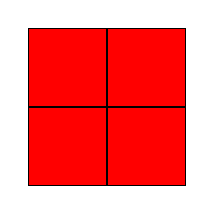
\begin{tikzpicture}
  \fill[red] (0,0) rectangle (2,2);
  \draw (0,0) rectangle (2,2);
  \draw (1,0) -- (1,2);
  \draw (0,1) -- (2,1);
\end{tikzpicture}
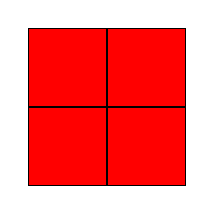
\begin{tikzpicture}
  \fill[red] (0,0) rectangle (2,2);
  \draw (0,0) rectangle (2,2);
  \draw (1,0) -- (1,2);
  \draw (0,1) -- (2,1);
\end{tikzpicture}
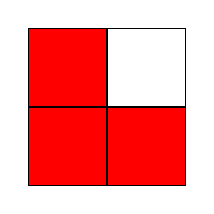
\begin{tikzpicture}
	  \fill[red] (0,0) rectangle (2,2);
	  \fill[white] (1,1) rectangle (2,2);
	  \draw (0,0) rectangle (2,2);
	  \draw (1,0) -- (1,2);
	  \draw (0,1) -- (2,1);
\end{tikzpicture}


\end{document}
